\chapter{Advanced Data Representation}
\label{chap:advanced_data_representation}

\begin{figure}[ht]
	\hfill
	\begin{minipage}{0.5\textwidth}
		\centering
		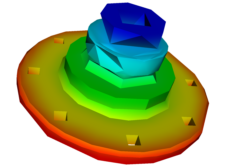
\includegraphics{VTKTextbook-158}\\
		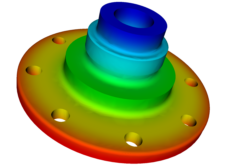
\includegraphics{VTKTextbook-157}
		\caption*{\texttt{Adaptive tessellation of higher-order cells.}}
	\end{minipage}
\end{figure}


\firstletter{T}his chapter examines advanced topics in data representation.
Topics include topological and geometric relationships and computational methods for cells and datasets.

\section{Coordinate Systems}
We will examine three different coordinate systems: the global, dataset, and structured coordinate systems.
Figure \ref{fig:Figure8-1} shows the relationship between the global and dataset coordinate systems, and depicts the structured coordinate system.

\begin{figure}[!htb]
	\centering
	\begin{subfigure}{0.48\linewidth}
		\centering
		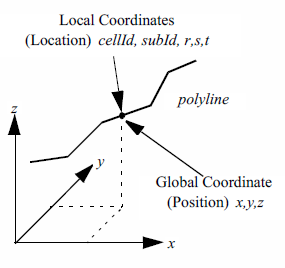
\includegraphics[width=\linewidth]{Figure8-1a}
		\caption*{}\label{fig:Figure8-1a}
	\end{subfigure}
	\hfill
	\begin{subfigure}{0.48\linewidth}
		\centering
		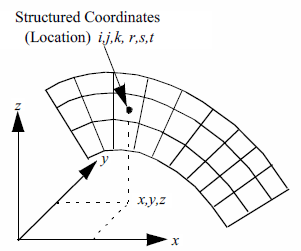
\includegraphics[width=\linewidth]{Figure8-1b}
		\caption*{}\label{fig:Figure8-1b}
	\end{subfigure}%
	\caption{Local and global coordinate systems.}
	\label{fig:Figure8-1}
\end{figure}


\subsection{Global Coordinate System}
The global coordinate system is a Cartesian, three-dimensional space. Each point is expressed as a triplet of values $(x,y,z)$ along the $x$, $y$, and $z$ axes.
This is the same system that was described in Chapter 3: \nameref{chap:computer_graphics_primer} (see \ref{sec:coordinate_systems}).
The global coordinate system is always used to specify dataset geometry (i.e., the point coordinates),and data attributes such as normals and vectors.
We will use the word ``position'' to indicate that we are using global coordinates.

\subsection{Dataset Coordinate System}

The dataset, or local, coordinate system is based on combined topological and geometric coordinates. The topological coordinate is used to identify a particular cell (or possibly a subcell), and the geometric coordinate is used to identify a particular location within the cell. Together they uniquely specify a location in the dataset. Here we will use the word ``location'' to refer to local or dataset coordinates.

The topological coordinate is an ``id'': a unique, nonnegative integer number referring to either a dataset point or cell. For a composite cell, we use an additional “sub-id” to refer to a particular primary cell that composes the composite cell. The sub-id is also unique and nonnegative. The id and sub-id together select a particular primary cell.

To specify a location within the primary cell, we use geometric coordinates. These geometric coordinates, or parametric coordinates, are coordinates ``natural'' or canonical to the particular topology and dimension of a cell.

We can best explain local coordinates by referring to an example. If we consider the polyline cell type shown in Figure \ref{fig:Figure8-2}, we can specify the position of a point by indicating 1) the polyline cell id, 2) the primary cell (i.e., line) sub-id and 3) the parametric coordinate of the line. Because the line is one-dimensional, the natural or parametric coordinate is based on the one-dimensional parameter r. Then any point along the line is given by a linear combination of the two end points of the line $x_i$ and $x_{i+1}$

\begin{equation}\label{eq:8.1}
x(r) = (1 - r) x_i + r x_{i + 1}
\end{equation}
\myequations{Parametric equation of a line.}

where the parametric coordinate $r$ is constrained between $(0,1)$. In this equation we are assuming that the sub-id is equal to $i$.

The number of parametric coordinates corresponds to the topological dimension of the cell. Three-dimensional cells will be characterized by the three parametric coordinates $(r, s, t)$. For cells of topological order less than three, we will ignore the last $(3 - n)$ parametric coordinates, where $n$ is the topological order of the cell. For convenience and consistency, we also will constrain each parametric coordinate to range between $(0,1)$.

Every cell type will have its own parametric coordinate system. Later in this chapter we will describe the parametric coordinate systems in detail. But first we will examine another coordinate system, the structured coordinate system.

\subsection{Structured Coordinate System}

Many dataset types are structured. This includes image data and structured grids. Because of their inherent structure, they have their own natural coordinate system. This coordinate system is based on the $i-j-k$ indexing scheme that we touched on in Chapter 5: \nameref{chap:basic_data_representation} (see``Image Data'' on page \pageref{subsec:image_data}).

The structured coordinate system is a natural way to describe components of a structured dataset. By fixing some indices, and allowing the others to vary within a limited range, we can specify points, lines, surfaces, and volumes. For example, by fixing the $i$ index $i = i_0$, and allowing the $j$ and $k$ indices to range between their minimum and maximum values, we specify a surface. If we fix three indices, we specify a point, if we fix two indices, we specify a line, and if we allow three indices to vary, we specify a volume (or sub-volume). The structured coordinate system is generally used to specify a region of interest (or ROI). The region of interest is an area that we want to visualize, or to operate on.

There is a simple relationship between the point and cell id of the dataset coordinate system and the structured coordinate system. To obtain a point id $p_\text{id}$ given the indices $(i_p, j_p, k_p)$ and dimensions $(n_x, n_y, n_z)$ we use

\begin{equation}\label{eq:8.2}
p_\text{id} = i_p +j_p n_x + k_p n_y
\end{equation}
\myequations{Obtaining a point id.}

with $0 \leq i_p \leq n_x, 0 \leq j_p \leq n_y, 0 \leq k_p \leq n_z$. (We can use this id to index into an array of points or point attribute data.) This equation implicitly assumes an ordering of the points in topological space. Points along the $i$ axis vary fastest, followed by the $j$ and then the $k$ axes. A similar relationship exists for cell id’s

\begin{equation}\label{eq:8.3}
\text{cell}_\text{id} = i_p + j_p (n_x - 1) + k_p (n_x - 1)(n_y - 1)
\end{equation}
\myequations{Obtaining a cell id.}

Here we’ve taken into account that there are one fewer cells along each topological axes than there are points.

\section{Interpolation Functions}
\label{sec:interpolation_functions}

Computer visualization deals with discrete data. The data is either supplied at a finite number of points or created by sampling continuous data at a finite number of points. But we often need information at positions other than these discrete point locations. This may be for rendering or for sub-sampling the data during algorithm execution. We need to interpolate data from known points to some intermediate point using interpolation functions.

Interpolation functions relate the values at cell points to the interior of the cell. Thus, we assume that information is defined at cell points, and that we must interpolate from these points. We can express the result as a weighted average of the data values at each cell point.

\begin{figure}[!htb]
	\centering
	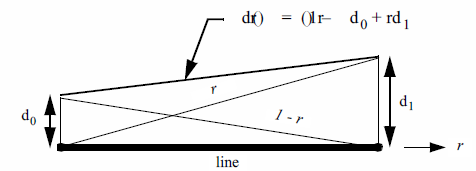
\includegraphics[width=0.98\textwidth]{Figure8-2}\\
	\caption{Interpolation is a linear combination of local interpolation functions. Interpolation functions are scaled by data values at cell points.}\label{fig:Figure8-2}
\end{figure}

\subsection{General Form}

To interpolate data from the cell points $p_i$ to a point $p$ that is inside the cell, we need three pieces of information:

\begin{itemize}

	\item the data values at each cell point,

	\item the parametric coordinates of the point $p$ within the cell, and

	\item the cell type including interpolation functions.

\end{itemize}

Given this information, the interpolation functions are a linear combination of the data values at the cell points

\begin{equation}\label{eq:8.4}
d = \sum_{i = 0}^{n - 1}W_i\,  d_i
\end{equation}
\myequations{Linear combination of data values at each cell point.}

where $d$ is the data value at the interior cell location $(r,s,t)$, $d_i$ is the data value at the $i^{th}$ cell point, and $W_i$ is a weight at the $i^{th}$ cell point. The interpolation weights are functions of the parametric coordinates $W_i = W(r,s,t)$. In addition, because we want $d = d_i$ when the interior point coincides with a cell point, we can place additional constraints on the weights

\begin{equation}\label{eq:8.5}
W_i = 1, W_{j \neq i} = 0 \quad \text{when} \quad p = p_i
\end{equation}
\myequations{Weighting constraints.}

We also desire the interpolated data value $d$ to be no smaller than the minimum $d_i$ and no larger than the maximum $d_i$. Thus the weights should also satisfy

\begin{equation}\label{eq:8.6}
\sum W_i = 1, \quad 0 \leq W_i \leq 1
\end{equation}
\myequations{Additional weighting constraints.}

The interpolation functions are of a characteristic shape. They reach their maximum value $W_i = 1$ at cell point $p_i$, and are zero at all other points. Examining Equation \ref{eq:8.1}, we draw Figure \ref{fig:Figure8-2} and see that each interpolation function has the shape of a peaked ``hat'', and that interpolation is a linear combination of these hat functions, scaled by the data value at each point.

Equation \ref{eq:8.4} is the general form for cell interpolation. It is used to interpolate any data value defined at the cell points to any other point within the cell. We have only to define the specific interpolation functions $W_i$ for each cell type.

\subsection{Specific Forms}

Each cell type has its own interpolation functions. The weights $W_i$ are functions of the parametric coordinates $r$, $s$, and $t$. In this section we will define the parametric coordinate system and interpolation function for each primary cell type. Composite cells use the interpolation functions and parametric coordinates of their composing primary cells. The only difference in coordinate system specification between primary and composite cells is that composite cells use the additional sub-id to specify a particular primary cell.

\begin{figure}[!htb]
	\centering
	\begin{subfigure}{0.48\linewidth}
		\centering
		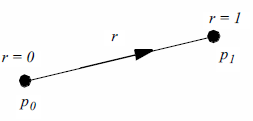
\includegraphics[width=\linewidth]{Figure8-3}
		\caption*{}
	\end{subfigure}
	\hfill
	\begin{subfigure}{0.48\linewidth}
		\centering
		\begin{equation*}
		\begin{array}{lll}
			W_0 &=& 1-r \\
			W_1 &=& r		
		\end{array}
		\end{equation*}
	\end{subfigure}%
	\caption{Parametric coordinate system and interpolation functions for a line.}
	\label{fig:Figure8-3}
\end{figure}

\begin{figure}[!htb]
	\centering
	\begin{subfigure}{0.48\linewidth}
		\centering
		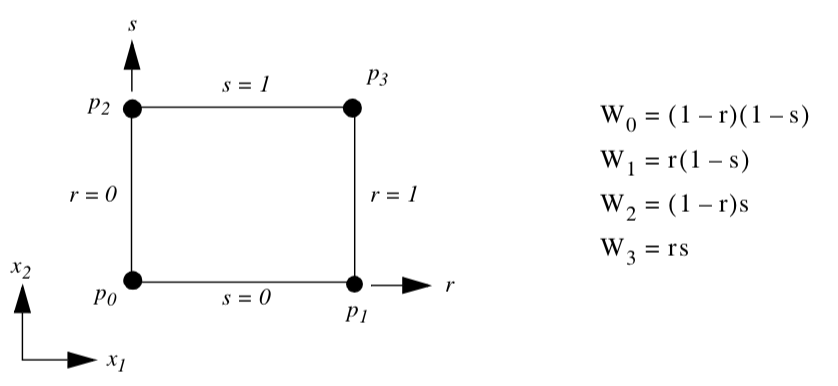
\includegraphics[width=\linewidth]{Figure8-4}
		\caption*{}
	\end{subfigure}
	\hfill
	\begin{subfigure}{0.48\linewidth}
		\centering
		\begin{equation*}
		\begin{array}{lll}
		W_0 &=& (1-r)(1 - s) \\
		W_1 &=& r(1 - s) \\
		W_2 &=& (1 - r)s \\
		W_3 &=& r s		
		\end{array}
		\end{equation*}
	\end{subfigure}%
	\caption{Parametric coordinate system and interpolation functions for a pixel.}
	\label{fig:Figure8-4}
\end{figure}

\begin{figure}[!htb]
	\centering
	\begin{subfigure}{0.48\linewidth}
		\centering
		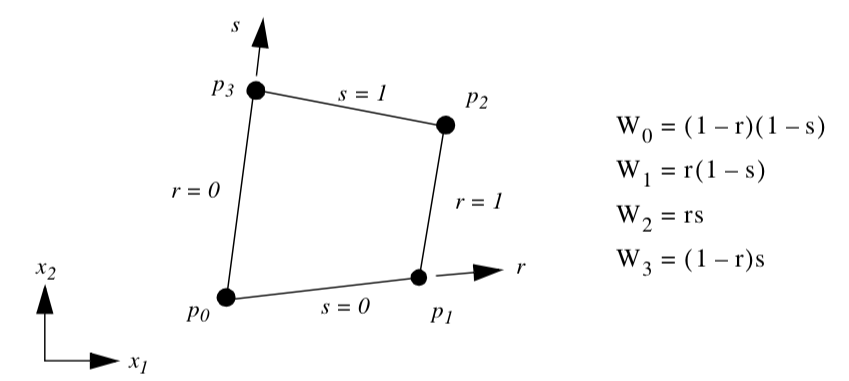
\includegraphics[width=\linewidth]{Figure8-5}
		\caption*{}
	\end{subfigure}
	\hfill
	\begin{subfigure}{0.48\linewidth}
		\centering
		\begin{equation*}
		\begin{array}{lll}
		W_0 &=& (1-r)(1 - s) \\
		W_1 &=& r(1 - s) \\
		W_2 &=& r s \\
		W_3 &=& (1 - r)s	
		\end{array}
		\end{equation*}
	\end{subfigure}%
	\caption{Parametric coordinate system and interpolation functions for a quadrilateral.}
	\label{fig:Figure8-5}
\end{figure}

\begin{figure}[!htb]
	\centering
	\begin{subfigure}{0.48\linewidth}
		\centering
		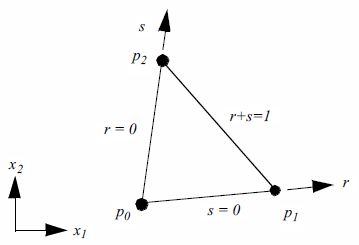
\includegraphics[width=\linewidth]{Figure8-6}
		\caption*{}
	\end{subfigure}
	\hfill
	\begin{subfigure}{0.48\linewidth}
		\centering
		\begin{equation*}
		\begin{array}{lll}
		W_0 &=& 1 - r - s \\
		W_1 &=& r \\
		W_2 &=& s 	
		\end{array}
		\end{equation*}
	\end{subfigure}%
	\caption{Parametric coordinate system and interpolation functions for a triangle.}
	\label{fig:Figure8-6}
\end{figure}

\begin{figure}[!htb]
	\centering
	\begin{subfigure}{0.48\linewidth}
		\centering
		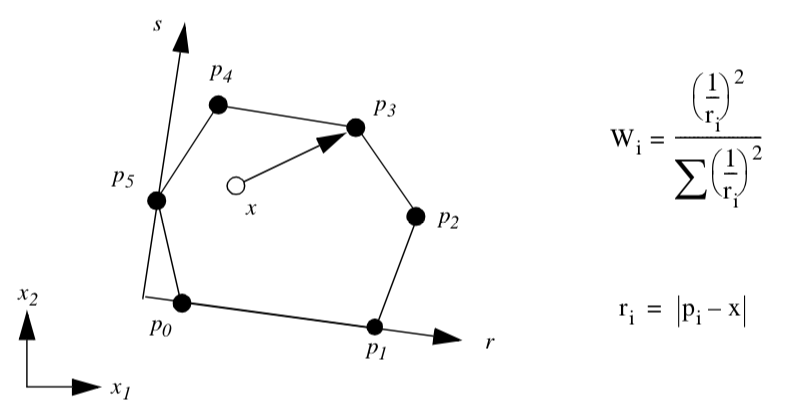
\includegraphics[width=\linewidth]{Figure8-7}
		\caption*{}
	\end{subfigure}
	\hfill
	\begin{subfigure}{0.48\linewidth}
		\centering
		\begin{equation*}
		\begin{array}{lll}
		W_i &=& \dfrac{r_i^{-2}}{\sum r_i^{-2}} \\ \\
		r_i &=& \vert p_i - x \vert	
		\end{array}
		\end{equation*}
	\end{subfigure}%
	\caption{Parametric coordinate system and interpolation functions for a polygon.}
	\label{fig:Figure8-7}
\end{figure}

\begin{figure}[!htb]
	\centering
	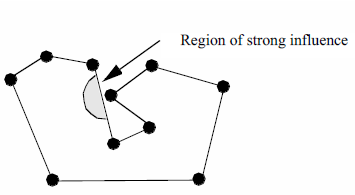
\includegraphics[width=0.48\textwidth]{Figure8-8}\\
	\caption{Potential problem with distance-based interpolation functions.}\label{fig:Figure8-8}
\end{figure}

\begin{figure}[!htb]
	\centering
	\begin{subfigure}{0.48\linewidth}
		\centering
		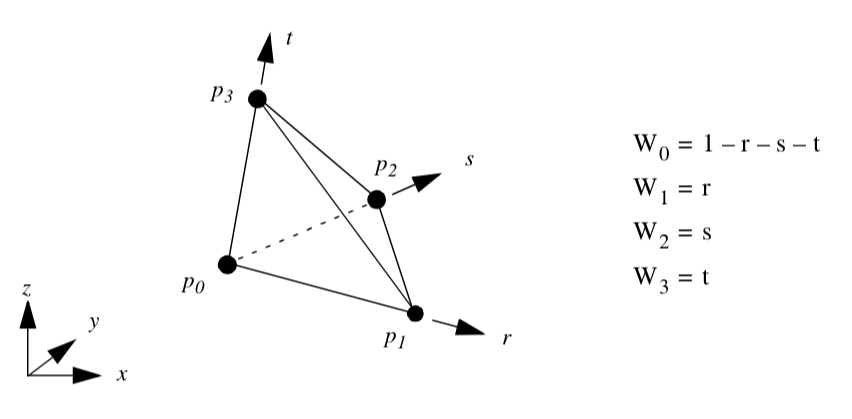
\includegraphics[width=\linewidth]{Figure8-9}
		\caption*{}
	\end{subfigure}
	\hfill
	\begin{subfigure}{0.48\linewidth}
		\centering
		\begin{equation*}
		\begin{array}{lll}
		W_0 &=& 1 - r - s - t \\
		W_1 &=& r \\
		W_2 &=& s \\
		W_3 &=& t	
		\end{array}
		\end{equation*}
	\end{subfigure}%
	\caption{Parametric coordinate system and interpolation functions for a tetrahedron.}
	\label{fig:Figure8-9}
\end{figure}

\begin{figure}[!htb]
	\centering
	\begin{subfigure}{0.48\linewidth}
		\centering
		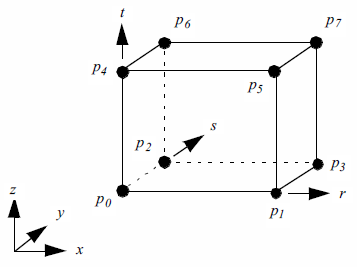
\includegraphics[width=\linewidth]{Figure8-10}
		\caption*{}
	\end{subfigure}
	\hfill
	\begin{subfigure}{0.48\linewidth}
		\centering
		\begin{equation*}
		\begin{array}{lll}
		W_0 &=& (1 - r)(1 - s)(1 - t) \\
		W_1 &=& r (1-s)(1 -t) \\
		W_2 &=& (1-r)s(1-t) \\
		W_3 &=& rs(1 - t) \\
		W_4 &=& (1 - r)(1 - s) t \\
		W_5 &=& r (1-s)t \\
		W_6 &=& (1 - r)s t \\
		W_7 &=& r s t	
		\end{array}
		\end{equation*}
	\end{subfigure}%
	\caption{Parametric coordinate system and interpolation functions for a tetrahedron.}
	\label{fig:Figure8-10}
\end{figure}

\begin{figure}[!htb]
	\centering
	\begin{subfigure}{0.48\linewidth}
		\centering
		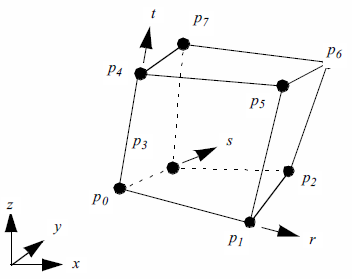
\includegraphics[width=\linewidth]{Figure8-11}
		\caption*{}
	\end{subfigure}
	\hfill
	\begin{subfigure}{0.48\linewidth}
		\centering
		\begin{equation*}
		\begin{array}{lll}
		W_0 &=& (1 - r)(1 - s)(1 - t) \\
		W_1 &=& r (1-s)(1 -t) \\
		W_2 &=& rs (1-t) \\
		W_3 &=& (1-r)s(1 - t) \\
		W_4 &=& (1 - r)(1 - s) t \\
		W_5 &=& r (1-s)t \\
		W_6 &=& rs t \\
		W_7 &=& (1-r)st	
		\end{array}
		\end{equation*}
	\end{subfigure}%
	\caption{Parametric coordinate system and interpolation functions for a hexahedron.}
	\label{fig:Figure8-11}
\end{figure}

\begin{figure}[!htb]
	\centering
	\begin{subfigure}{0.48\linewidth}
		\centering
		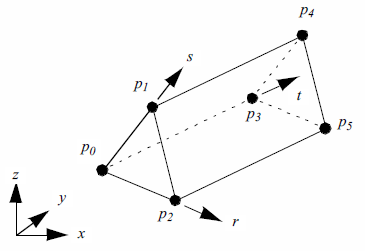
\includegraphics[width=\linewidth]{Figure8-12}
		\caption*{}
	\end{subfigure}
	\hfill
	\begin{subfigure}{0.48\linewidth}
		\centering
		\begin{equation*}
		\begin{array}{lll}
		W_0 &=& (1 - r - s)(1 - t) \\
		W_1 &=& r (1-t) \\
		W_2 &=& s (1 - t) \\
		W_3 &=& (1 - r - s)t \\
		W_4 &=& r t \\
		W_5 &=& s t	
		\end{array}
		\end{equation*}
	\end{subfigure}%
	\caption{Parametric coordinate system and interpolation functions for a wedge.}
	\label{fig:Figure8-12}
\end{figure}

\begin{figure}[!htb]
	\centering
	\begin{subfigure}{0.48\linewidth}
		\centering
		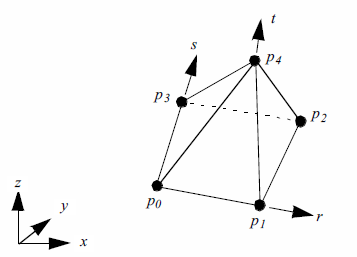
\includegraphics[width=\linewidth]{Figure8-13}
		\caption*{}
	\end{subfigure}
	\hfill
	\begin{subfigure}{0.48\linewidth}
		\centering
		\begin{equation*}
		\begin{array}{lll}
		W_0 &=& (1-r)(1-s)(1-t) \\
		W_1 &=& r(1-s)(1-t) \\
		W_2 &=& r s (1-t) \\
		W_3 &=& (1-r)s(1-t) \\
		W_4 &=& t	
		\end{array}
		\end{equation*}
	\end{subfigure}%
	\caption{Parametric coordinate system and interpolation functions for a pyramid.}
	\label{fig:Figure8-13}
\end{figure}

\begin{figure}[!htb]
	\centering
	\begin{subfigure}{0.48\linewidth}
		\centering
		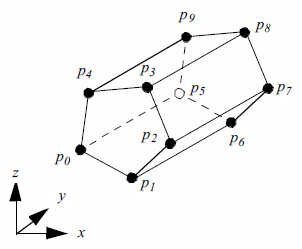
\includegraphics[width=\linewidth]{Figure8-14a}
		\caption*{}
	\end{subfigure}
	\hfill
	\begin{subfigure}{0.48\linewidth}
		\centering
		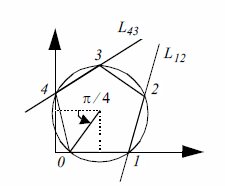
\includegraphics[width=\linewidth]{Figure8-14b}
		\caption*{}
	\end{subfigure}
	\hfill
	\begin{subfigure}{0.48\linewidth}
		\centering
		\begin{equation*}
		\begin{array}{lll}
		W_0 &=& -N(-As + Br - C)(Bs-Ar-C)(t - 1) \\
		W_1 &=& N(Ds+Dr-E)(Fs-Gr-H)(t-1) \\
		W_2 &=& -N(Bs -Ar -C)(-Gs-Fr+H)(t - 1)\\
		W_3 &=& N(-As + Br -C)(Fs + Gr - H)(t - 1) \\
		W_4 &=& -N(-Gs - Fr + H)(Ds + Dr - E)(t - 1) \\
		W_5 &=& N(-As +Br - C)(Bs -Ar -C)t \\
		W_6 &=& -N(Ds + Dr - E)(Fs + Gr - H)t\\
		W_7 &=& N(Bs - Ar -C)(-Gs -Fr + H)t \\
		W_8 &=& -N(-As + Br -C)(Fs + Gr - H)t \\
		W_9 &=& N(-Gs - Fr + H)(Ds + Dr -E)t
		\end{array}
		\end{equation*}
	\end{subfigure}%
	\hfill
	\begin{subfigure}{0.48\linewidth}
		\centering
		The points $P_i(x_i, y_i)$ on the pentagon are defined by:
		\begin{equation*}
		\begin{array}{lll}
		x_i &=& \dfrac{1}{2}\left(1 +\cos\left(\dfrac{5\pi}{4} + i \dfrac{2\pi}{5}\right)\right) \\ \\
		y_i &=& \dfrac{1}{2}\left(1 +\sin\left(\dfrac{5\pi}{4} + i \dfrac{2\pi}{5}\right)\right) \\ \\
		i &\in& \lbrace 0, 1, 2, 3, 4 \rbrace
		\end{array}
		\end{equation*}
		Constants:
		\begin{equation*}
		\begin{array}{lll}
		A &=& x_2 - x_1 \\
		B &=& y_2 - y_1 \\
		C &=& x_1 y_2 - x_2 y_1 \\
		D &=& x_2 - x_3 \\
		E &=& x_2 y_3 - x_3 y_2 \\
		F &=& x_0 - x_4 \\
		G &=& y_4 - y_0 \\
		H &=& x_0 y_4 - x_4 y_0	
		\end{array}
		\end{equation*}
	\end{subfigure}%
	\caption{Parametric coordinate system and interpolation functions for a pentagonal prism.}
	\label{fig:Figure8-14}
\end{figure}

\begin{figure}[!htb]
	\centering
	\begin{subfigure}{0.48\linewidth}
		\centering
		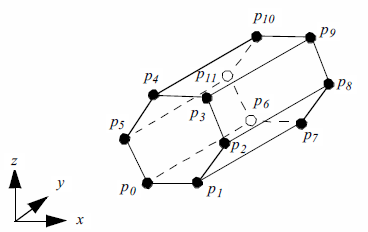
\includegraphics[width=\linewidth]{Figure8-15}
		\caption*{}
	\end{subfigure}
	\hfill
	\begin{subfigure}{0.48\linewidth}
		\centering
		\begin{equation*}
		\begin{array}{lll}
		\alpha &=& \dfrac{\sqrt{3}}{4} + \dfrac{1}{2} \\ \\
		\beta &=& \dfrac{1}{2} - \dfrac{\sqrt{3}}{4}, \alpha + \beta = 1
		\end{array}
		\end{equation*}
	\end{subfigure}
	\hfill
	\begin{subfigure}{0.48\linewidth}
		\centering
		\begin{equation*}
		\begin{array}{lll}
		W_0 &=&-\dfrac{16}{3}(r - \alpha)(r - \beta)(s - 1)(t - 1) \\ \\
		W_1 &=&\dfrac{16}{3}(r - \dfrac{1}{2})(r - \beta)(s - \dfrac{3}{4})(t - 1) \\ \\
		W_2 &=& -\dfrac{16}{3}(r - \dfrac{1}{2})(r - \beta)(s - \dfrac{1}{4})(t - 1) \\ \\
		W_3 &=& \dfrac{16}{3}(r - \alpha)(r - \beta)s(t - 1) \\ \\
		W_4 &=& -\dfrac{16}{3}(r - \dfrac{1}{2})(r - \alpha)(s - \dfrac{1}{4})(t - 1) \\ \\
		W_5 &=& \dfrac{16}{3}(r - \dfrac{1}{2})(r - \alpha)(s - \dfrac{3}{4})(t - 1)
		\end{array}
		\end{equation*}
	\end{subfigure}%
	\hfill
	\begin{subfigure}{0.48\linewidth}
		\centering
		\begin{equation*}
		\begin{array}{lll}
		W_6 &=& \dfrac{16}{3}(r - \alpha)(r - \beta)(s - 1)t \\ \\
		W_7 &=&-\dfrac{16}{3}(r - \dfrac{1}{2})(r - \beta)(s - \dfrac{3}{4})t \\ \\
		W_8 &=&  \dfrac{16}{3}(r - \dfrac{1}{2})(r - \beta)(s - \dfrac{1}{4})t \\ \\
		W_9 &=& -\dfrac{16}{3}(r - \alpha)(r - \beta)st \\ \\
		W_{10} &=&  \dfrac{16}{3}(r - \dfrac{1}{2})(r - \alpha)(s - \dfrac{1}{4})t \\ \\
		W_{11} &=& -\dfrac{16}{3}(r - \dfrac{1}{2})(r - \alpha)(s - \dfrac{3}{4})t
		\end{array}
		\end{equation*}
	\end{subfigure}%
\caption{Parametric coordinate system and interpolation functions for a hexagonal prism.}
\label{fig:Figure8-15}
\end{figure}

\begin{figure}[!htb]
	\centering
	\begin{subfigure}{0.48\linewidth}
		\centering
		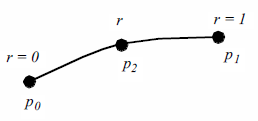
\includegraphics[width=\linewidth]{Figure8-16}
		\caption*{}
	\end{subfigure}
	\hfill
	\begin{subfigure}{0.48\linewidth}
		\centering
		\begin{equation*}
		\begin{array}{lll}
		W_0 &=& 2 \left( r - \dfrac{1}{2}\right)(r - 1) \\ \\
		W_1 &=& 2 r \left( r - \dfrac{1}{2}\right) \\ \\
		W_2 &=& 4 r (1 - r)	
		\end{array}
		\end{equation*}
	\end{subfigure}%
	\caption{Parametric coordinate system and interpolation functions for a quadratic wedge.}
	\label{fig:Figure8-16}
\end{figure}

\begin{figure}[!htb]
	\centering
	\begin{subfigure}{0.48\linewidth}
		\centering
		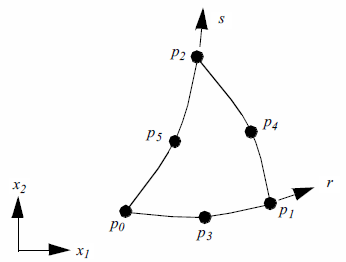
\includegraphics[width=\linewidth]{Figure8-17}
		\caption*{}
	\end{subfigure}
	\hfill
	\begin{subfigure}{0.48\linewidth}
		\centering
		\begin{equation*}
		\begin{array}{lll}
		W_0 &=& (1 - r - s)(2(1 - r - s) - 1) \\
		W_1 &=& r (2 r - 1) \\
		W_2 &=& s(2s - 1) \\
		W_3 &=& 4 r (1 - r - s) \\
		W_4 &=& 4 r s \\
		W_5 &=& 4 s (1 - r - s)	
		\end{array}
		\end{equation*}
	\end{subfigure}%
	\caption{Parametric coordinate system and interpolation functions for a quadratic triangle.}
	\label{fig:Figure8-17}
\end{figure}

\begin{figure}[!htb]
	\centering
	\begin{subfigure}{0.48\linewidth}
		\centering
		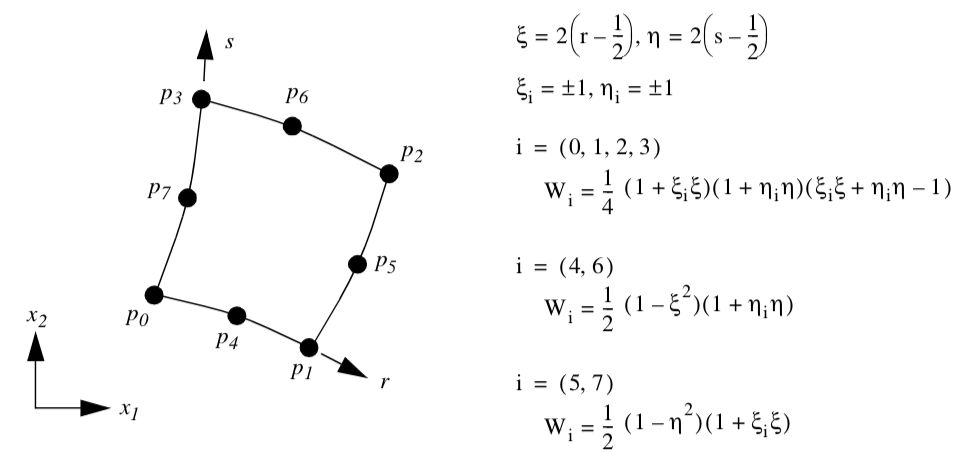
\includegraphics[width=\linewidth]{Figure8-18}
		\caption*{}
	\end{subfigure}
	\hfill
	\begin{subfigure}{0.48\linewidth}
		\centering
		\begin{equation*}
		\begin{array}{lll}
		\xi &=& 2 r  - 1, \quad \xi_i = \pm 1 \\
		\eta &=& 2 s - 1, \quad \eta_i = \pm 1
		\end{array}
		\end{equation*}
		\begin{equation*}
		\begin{array}{lll}
		W_i &=& (1 + \xi_i \xi)(1 + \eta_i \eta)(\xi_i \xi + \eta_i \eta - 1)/4, \\
		i &\in& \lbrace 0, 1, 2, 3, 4 \rbrace \\ \\
		W_i &=& (1 - \xi^2)(1 + \eta_i \eta)/2,\\
		i &\in& \lbrace 4, 6 \rbrace  \\ \\
		W_i &=& (1 - \eta^2)(1 + \xi_i \xi)/2, \\
		i &\in& \lbrace 5, 7 \rbrace	
		\end{array}
		\end{equation*}
	\end{subfigure}%
	\caption{Parametric coordinate system and interpolation functions for a quadratic quadrilateral. In VTK parametric coordinates $(r,s)$ run between (0,1), hence the coordinate system shift into the $(\xi, \eta$) parametric system ranging from $(-1,1)$. Note that $\xi_i$ and $\eta_i$ refer to the parametric coordinates of the $i^{th}$ point.}
	\label{fig:Figure8-18}
\end{figure}


\begin{figure}[!htb]
	\centering
	\begin{subfigure}{0.48\linewidth}
		\centering
		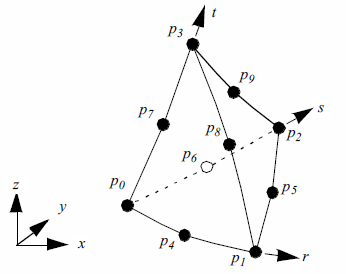
\includegraphics[width=\linewidth]{Figure8-19}
		\caption*{}
	\end{subfigure}
	\hfill
	\begin{subfigure}{0.48\linewidth}
		\centering
		\begin{equation*}
		\begin{array}{lll}
		u &=& 1 - r - s- t \\ \\
		W_0 &=& u(2u-1) \\
		W_1 &=& r(2r - 1) \\
		W_2 &=& s(2s - 1) \\
		W_3 &=& t (2t - 1)	
		\end{array}
		\end{equation*}
		\noindent\begin{minipage}{.5\linewidth}
			\begin{equation*}
			\begin{array}{lll}
			W_4 &=& 4 u r \\
			W_5 &=& 4 r s \\
			W_6 &=& 4 s u	
			\end{array}
			\end{equation*}
		\end{minipage}%
		\noindent\begin{minipage}{.5\linewidth}
			\begin{equation*}
			\begin{array}{lll}
			W_7 &=& 4 u t \\
			W_8 &=& 4 r t \\
			W_9 &=& 4 s t	
			\end{array}
			\end{equation*}
		\end{minipage}%
		
	\end{subfigure}%
	\caption{Parametric coordinate system and interpolation functions for a quadratic tetrahedron. In VTK parametric coordinates $(r,s,t)$ run between $(0,1)$, hence the coordinate system shift into the $(\xi, \eta, \zeta)$ parametric system ranging from $(-1,1)$.}
	\label{fig:Figure8-19}
\end{figure}

\begin{figure}[!htb]
	\centering
	\begin{subfigure}{0.48\linewidth}
		\centering
		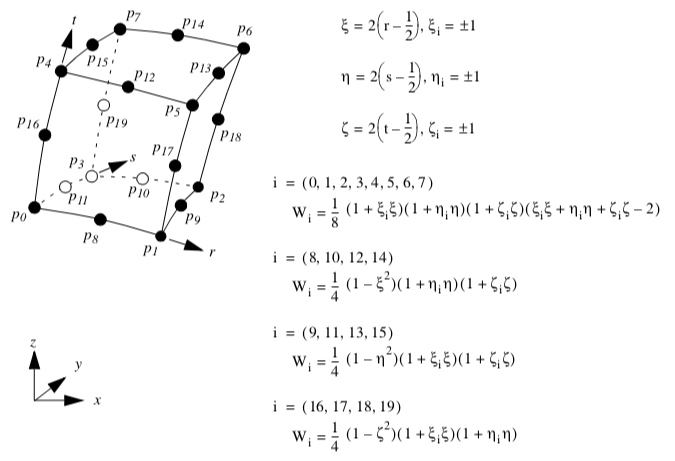
\includegraphics[width=\linewidth]{Figure8-20}
		\caption*{}
	\end{subfigure}
	\hfill
	\begin{subfigure}{0.48\linewidth}
		\begin{equation*}
		\begin{array}{lll}
		\xi &=& 2r  - 1,\quad \xi_i = \pm1 \\
		\eta &=& 2 s - 1,\quad \eta_i = \pm1 \\
		\zeta &=& 2 t - 1,\quad \zeta_i = \pm1
		\end{array}
		\end{equation*}
		\begin{equation*}
		\begin{array}{lll}
		W_i &=& (1 + \xi_i \xi)(1 + \eta_i \eta)(1 + \zeta_i \zeta)(\xi_i \xi + \eta_i \eta + \zeta_i \zeta - 2)/8, \\
		i &\in& \lbrace 1 \ldots 7 \rbrace \\ \\
		W_i &=& (1 - \xi^2)(1 + \eta_i \eta)(1 + \zeta_i \zeta)/4, \\
		i &\in& \lbrace 8, 10, 12, 14 \rbrace \\ \\
		W_i &=& (1 - \eta^2)(1 + \xi_i \xi)(1 + \zeta_i \zeta)/4, \\
		i &\in& \lbrace 9, 11, 13, 15 \rbrace \\ \\
		W_i &=& (1 - \zeta^2)(1 + \xi_i \xi)(1 + \eta_i \eta)/4, \\
		i &\in& \lbrace 16, 17, 18, 19 \rbrace	
		\end{array}
		\end{equation*}		
	\end{subfigure}%
	\caption{Parametric coordinate system and interpolation functions for a quadratic hexahedron. In VTK parametric coordinates $(r,s,t)$ run between $(0,1)$, hence the coordinate system shift into the $(\xi, \eta, \zeta)$ parametric system ranging from (-1,1). Note that $\xi_i$, $\eta_i$ and $\zeta_i$ refer to the parametric coordinates of the $i^{th}$ point.}
	\label{fig:Figure8-20}
\end{figure}

\begin{figure}[!htb]
	\centering
	\begin{subfigure}{0.48\linewidth}
		\centering
		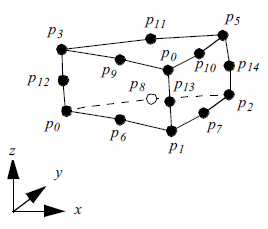
\includegraphics[width=\linewidth]{Figure8-21}
		\caption*{}
	\end{subfigure}
	\hfill
	\begin{subfigure}{0.48\linewidth}
		\centering
		\begin{equation*}
		\begin{array}{lll}
		W_0 &=& (1 - r - s)(1 - t)(1 - 2r -2s -2t) \\
		W_1 &=& r(1 - t)(2r - 2t - 1) \\
		W_2 &=& s(1 - t)(2s - 2t - 1) \\
		W_3 &=& (1 - r - s)t(2t - 2r - 2s - 1) \\
		W_4 &=& rt(2r + 2t - 3) \\
		W_5 &=& st(2s + 2t - 3) \\
		W_6 &=& 4r(1 - r - s)(1 - t) \\
		W_7 &=& 4rs(1 - t) \\
		W_8 &=& 4s(1 - t)(1 - r - s) \\
		W_9 &=& 4r(1 - r - s)t \\
		W_{10} &=& 4 rst \\
		W_{11} &=& 4 (1 - r - s)s t\\
		W_{12} &=& 4 (1 - r - s)t(1 - t) \\
		W_{13} &=& 4rt(1 - t) \\
		W_{14} &=& 4st(1 - t)	
		\end{array}
		\end{equation*}
	\end{subfigure}%
	\caption{Parametric coordinate system and interpolation functions for a quadratic wedge.}
	\label{fig:Figure8-21}
\end{figure}

\begin{figure}[!htb]
	\centering
	\begin{subfigure}{0.48\linewidth}
		\centering
		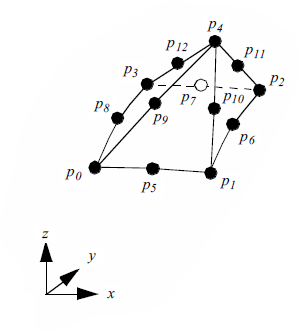
\includegraphics[width=\linewidth]{Figure8-22}
		\caption*{}
	\end{subfigure}
	\hfill
	\begin{subfigure}{0.48\linewidth}
		\centering
		\begin{equation*}
		\begin{array}{lll}
		\xi &=& 2 r - 1, \quad \xi_i = \pm1 \\ \\
		\eta &=& 2 s - 1, \quad \eta_i = \pm1 \\ \\
		\zeta &=& 2 t - 1, \quad \zeta_i = \pm1
		\end{array}
		\end{equation*}
		\begin{equation*}
		\begin{array}{lll}
		W_i &=& (1 + \xi_i \xi)(1 + \eta_i \eta)(1 + \zeta_i \zeta)(\xi_i \xi + \eta_i \eta + \zeta_i \zeta - 2)/8, \\
		i &\in& \lbrace 0, 1, 2, 3 \rbrace \\
		W_4 &=& \zeta(1 - \zeta)/4, \quad i \in \lbrace 4 \rbrace \\
		W_i &=& (1 - \xi^2)(1 + \eta_i \eta)(1 + \zeta_i \zeta)/4, \quad i \in \lbrace 5, 6, 7, 8\rbrace \\
		W_i &=& (1 - \zeta^2)(1 + \xi_i \xi)(1 + \eta_i \eta)/4, \quad i \in \lbrace 9, 10, 11, 12 \rbrace	
		\end{array}
		\end{equation*}
	\end{subfigure}%
	\caption{Parametric coordinate system and interpolation functions for a quadratic pyramid. In VTK parametric coordinates $(r,s,t)$ run between $(0,1)$, hence the coordinate system shift into the $(\xi, \eta, \zeta)$ parametric system ranging from (-1,1). Note that $\xi_i$, $\eta_i$ and $\zeta_i$ refer to the parametric coordinates of the $i^{th}$ point.}
	\label{fig:Figure8-22}
\end{figure}


\section{Searching}
\label{sec:searching}
Searching is an operation to find the cell containing a specified point \emph{p}, or to locate cells or points in a region surrounding \emph{p}.
Algorithms requiring this operation include streamline generation, where we need to find the starting location within a cell; probing, where the data values at a point are interpolated from the containing cell; or collision detection, where cells in a certain region must be evaluated for intersection.
Sometimes (e.g., image datasets), searching is a simple operation because of the regularity of data. However, in less structured data, the searching operation is more complex.

To find the cell containing \emph{p}, we can use the following naive search procedure.
Traverse all cells in the dataset, finding the one (if any) that contains \emph{p}.
To determine whether a cell contains a point, the cell interpolation functions are evaluated for the parametric coordinates $(r,s,t)$.
If these coordinates lie within the cell, then \emph{p} lies in the cell.
The basic assumption here is that cells do not overlap, so that at most a single cell contains the given point \emph{p}.
To determine cells or points lying in the region surrounding \emph{p}, we can traverse cells or points to see whether they lie within the region around \emph{p}.
For example, we can choose to define the region as a sphere centered at \emph{p}.
Then, if a point or the points composing a cell lie in the sphere, the point or cell is considered to be in the region surrounding \emph{p}.

\section{Putting It All Together}
In this section we will finish our earlier description of an implementation for unstructured data. We also define a high-level, abstract interface for cells and datasets. This interface allows us to implement the general (i.e., dataset specific) algorithms in the \emph{Visualization Toolkit}. We also describe
implementations for color scalars, searching and picking, and conclude with a series of examples to demonstrate some of these concepts.

\subsection{Picking}
\label{subsec:picking}

The Visualization Toolkit provides a variety of classes to perform actor (or vtkProp), point, cell, and
world point picking ( Figure8–38 ).

\subsection{Point Probe}
\label{subsec:point_probe}

\section{Chapter Summary}

Three important visualization coordinate systems are the world, dataset, and structured coordinate systems. The world coordinate system is an x--y--z Cartesian three-dimensional space. The dataset coordinate system consists of a cell id, subcell id, and parametric coordinates. The structured coordinate system consists of $(i,j,k)$ integer indices into a rectangular topological domain.

Visualization data is generally in discrete form. Interpolation functions are used to obtain data at points between the known data values. Interpolation functions vary depending on the particular cell type. The form of the interpolation functions are weighting values located at each of the cells points. The interpolations functions form the basis for conversion from dataset to global coordinates and vice versa. The interpolation functions also are used to compute data derivatives.

Topological operators provide information about the topology of a cell or dataset. Obtaining neighboring cells to a particular cell is an important visualization operation. This operation can be used to determine whether cell boundaries are on the boundary of a dataset or to traverse datasets on a cell-by-cell basis.

Because of the inherent regularity of image datasets, operations can be efficiently implemented compared to other dataset types. These operations include coordinate transformation, derivative computation, topological query, and searching.

\section{Bibliographic Notes}

Interpolation functions are employed in a number of numerical techniques. The finite element method, in particular, depends on interpolation functions. If you want more information about interpolation functions refer to the finite element references suggested below \cite{Cook89} \cite{Gallagher75} \cite{Zienkiewicz87}. These texts also discuss derivative computation in the context of interpolation functions.

Visualizing higher-order datasets is an oepn research issue. While \cite{Schroeder06} describes one approach, methods based on GPU programs are emerging. Other approaches include tailored algorithms for a particular cell type.

Basic topology references are available from a number of sources. Two good descriptions of topological data structures are available from Weiler \cite{Weiler86} \cite{Weiler88} and Baumgart \cite{Baumgart74}. Weiler describes the radial-edge structure. This data structure can represent manifold and nonmanifold geometry. The winged-edge structure described by Baumgart is widely known. It is used to represent manifold geometry. Shephard \cite{Shephard88} describes general finite element data structures — these are similar to visualization structures but with extra information related to analysis and geometric modelling.

There are extensive references regarding spatial search structures. Samet \cite{Samet90} provides a general overview of some. Octrees were originally developed by Meagher \cite{Meagher82} for 3D imaging. See \cite{Williams83}, \cite{Bentley75}, and \cite{Quinlan94} for information about MIP maps, kd-trees, and binary sphere trees, respectively.

\printbibliography


\section{Exercises}